%-----------------------------------------------------------------------
\section{Kinematics of the fold}
\label{sec:kinematics}
%-----------------------------------------------------------------------

This section is the foundation the rest of the paper stands on. It defines the
scene, derives the map from surface positions to receiver positions, states
exactly what irradiance that map induces, and then establishes the statements
about the fold that matter for rendering: that its density is unbounded, that
it has a normal form, that the normal form yields the wavelength scaling, and
that the resulting intensity cannot be normalised by a constant.

\subsection{The scene}
\label{sec:scene}

The test configuration is a circular glass cylinder, a water column inside it,
and a matte receiver, lit by a distant source. The parameters are fixed for the
whole paper and are listed in Table~\ref{tab:scene}; Figure~\ref{fig:scene}
draws the arrangement to scale.

\begin{table}[t]
\centering
\caption{Scene parameters. The material models are the measured forms of
Section~\ref{sec:dispersion}, not fits. The source angular diameter is the true
solar value, which sets a coherence scale far larger than the fringe spacing
this paper is about --- see the remark in Section~\ref{sec:limits-coherence}.}
\label{tab:scene}
\small
\begin{tabular}{@{}lll@{}}
\toprule
Quantity & Value & Note \\
\midrule
Glass outer radius        & \SI{35}{\milli\meter}       & cylinder \\
Glass wall thickness      & \SI{3.5}{\milli\meter}      & \\
Glass height              & \SI{90}{\milli\meter}       & \\
Water fill height         & \SI{59.4}{\milli\meter}     & \\
Receiver                  & \SI{320}{\milli\meter}$^2$ patch & matte, Lambertian \\
Source                    & \SI{0.53}{\degree}          & distant, solar \\
Water index               & \num{1.33167} / \num{1.33468} / \num{1.33961} & R/G/B \\
Glass index               & \num{1.52104} / \num{1.52514} / \num{1.53192} & R/G/B \\
Channels                  & \SI{650}{} / \SI{550}{} / \SI{450}{\nano\meter} & R/G/B \\
\bottomrule
\end{tabular}
\end{table}

\begin{figure*}[t]
\centering
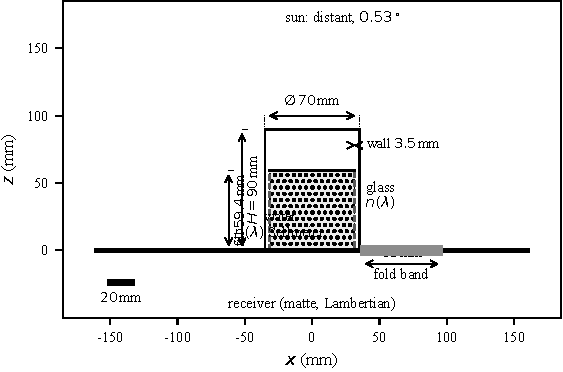
\includegraphics[width=\textwidth]{figures/fig1_scene.pdf}
\caption{The test scene drawn to scale. The glass body, water column, wall
thickness, fill height and receiver are shown at true relative size with
dimension lines; the ray path is traced through the actual geometry of
Section~\ref{sec:scene} at the central channel index rather than sketched. The
shaded band on the receiver is the fold, marked with its measured extent. All
lengths in millimetres.}
\label{fig:scene}
\end{figure*}

\subsection{The surface and its normal}
\label{sec:surface}

Let the water surface be a height field over $\mathbf{x} = (x,y) \in
\mathbb{R}^2$,
\begin{equation}
h(\mathbf{x},t) \;=\; \sum_{i=1}^{4} A_i \sin\!\big(k_i\,(\hat{\mathbf{u}}_i
\cdot \mathbf{x}) - \omega_i t\big),
\qquad k_i = \frac{2\pi}{\Lambda_i},
\label{eq:surface}
\end{equation}
a sum of four directional sinusoids with amplitudes $A_i = \{0.65, 0.40, 0.25,
0.15\}\,\si{\milli\meter}$ at wavelengths $\Lambda_i = \{42, 27, 17,
11\}\,\si{\milli\meter}$. The expansion in \eqref{eq:surface} is convenient
rather than essential: nothing below uses the sinusoidal form except to know
that $\nabla h$ is analytic and that $|\nabla h|$ is small. The outward normal
follows from the analytic gradient,
\begin{equation}
\nrm(\mathbf{x},t) \;=\; \frac{(-\partial_x h,\; -\partial_y h,\; 1)}
{\sqrt{1 + |\nabla h|^2}} .
\label{eq:normal}
\end{equation}

\begin{remark}[The slope is the small parameter]
\label{rem:slope}
For the amplitudes above, $|\nabla h| \le \sum_i A_i k_i \approx 0.34$ at the
shortest wave, so the surface stays well inside the small-slope regime in which
the paraxial normal form of Section~\ref{sec:foldnormal} is the leading term.
This matters because the fold normal form is asymptotic, and a surface steep
enough to produce higher-order caustics would leave its domain of validity. We
return to this in Section~\ref{sec:limits-fold}.
\end{remark}

\subsection{The ray map}
\label{sec:raymap}

Let the source direction be the unit vector $\dir$ pointing along propagation
(downward, into the surface). Vector Snell refraction at the interface gives the
transmitted direction. With the ratio $\eta = n_1/n_2$ and the cosine of
incidence $c_i = -\dir \cdot \nrm > 0$,
\begin{equation}
\trn \;=\; \eta\,\dir + \big(\eta\,c_i - \sqrt{1 - \eta^2(1 - c_i^2)}\big)\,\nrm ,
\qquad \eta^2(1-c_i^2) \le 1 ,
\label{eq:snell}
\end{equation}
where the inequality failing signals total internal reflection and the sample
carries no transmitted power. A refracted ray leaves the surface at height
$h(\mathbf{x})$ and reaches the receiver plane at $z = -D$ after a path length
$s = (-D - h(\mathbf{x}))/\hat t_z$. Composing the two gives the
\emph{surface-to-receiver ray map}
\begin{equation}
\Hm(\mathbf{x}) \;=\; \mathbf{x} + \trn(\mathbf{x})\,
\frac{-D - h(\mathbf{x})}{\hat t_z(\mathbf{x})},
\qquad
\Hm : \mathbb{R}^2 \to \mathbb{R}^2 .
\label{eq:raymap}
\end{equation}
Write $\Jm = \partial \Hm / \partial \mathbf{x}$ for its Jacobian and
$\detJ$ for its determinant. For the scene of Table~\ref{tab:scene},
$\Hm$ is a smooth map on the region of the surface that is not shadowed and not
totally reflecting.

\subsection{What the map induces on the receiver}
\label{sec:pushforward}

Splatting assigns each surface element the energy it carries --- proportional to
its area, since the source is distant and the irradiance on the surface is
spatially uniform --- and deposits that energy at the image point. The resulting
receiver irradiance is therefore the push-forward of the surface measure under
$\Hm$:
\begin{equation}
I(\mathbf{u}) \;=\; \sum_{\mathbf{x}\,:\,\Hm(\mathbf{x}) = \mathbf{u}}
\frac{1}{\big|\detJ(\mathbf{x})\big|} ,
\label{eq:irradiance}
\end{equation}
where the sum runs over the preimages of $\mathbf{u}$, which is the standard
sum over branches of a multi-valued inverse. It is worth being precise about the
status of \eqref{eq:irradiance}: it is exact for the geometric model, not an
estimator. Every method in Section~\ref{sec:cg} estimates this same object, and
that shared target is why they share a failure.

\begin{remark}[Why the determinant and not a solid angle]
\label{rem:det}
Equation~\eqref{eq:irradiance} is the Jacobian form of the usual
$\cos\theta / r^2$ falloff; the same determinant is what Arvo
\cite{arvo1994} propagates irradiance with in a different setting, which is why
the degeneracy studied here is a familiar object. The two agree wherever $\Hm$ is a diffeomorphism;
\eqref{eq:irradiance} is preferable here because it remains meaningful as a
statement about rank, which is what the fold is about.
\end{remark}

\subsection{The fold, and why a quadrature fails there}
\label{sec:fold}

\begin{definition}[Fold locus]
\label{def:fold}
The \emph{fold locus} of the scene is
$\fold = \{\,\mathbf{x} : \detJ(\mathbf{x}) = 0\,\}$, and its image
$\Hm(\fold)$ is the caustic curve on the receiver.
\end{definition}

\begin{assumption}[Generic fold]
\label{as:fold}
Throughout, we assume the degenerate points of $\Hm$ are folds: that
$\detJ = 0$ on $\fold$, that $\nabla \detJ \neq 0$ there, and that
$\operatorname{rank} \Jm = 1$ on $\fold$. Cusps, where $\nabla \detJ$ also
vanishes, are excluded and are discussed in Section~\ref{sec:limits-fold}.
\end{assumption}

\begin{lemma}[The fold density is unbounded]
\label{lem:diverge}
Let Assumption~\ref{as:fold} hold, and let $\mathbf{x}_0 \in \fold$. Let
$\mu$ be the push-forward of surface area under $\Hm$. Then the density of
$\mu$ with respect to Lebesgue measure on the receiver is unbounded in every
neighbourhood of $\Hm(\mathbf{x}_0)$.
\end{lemma}

\begin{proof}
By Whitney's normal form for a rank-one map \cite{whitney1955,golubitsky1986},
there are local coordinates $(u,v)$ near $\mathbf{x}_0$ and $(a,b)$ near
$\Hm(\mathbf{x}_0)$ in which $\Hm$ takes the form
\begin{equation}
\Hm(u,v) \;=\; (u,\; v^2) .
\label{eq:normalform}
\end{equation}
This is legitimate because Assumption~\ref{as:fold} puts us in the stable
one-fold stratum, and the normal form is stable under perturbation, so it
describes the map in a neighbourhood rather than only at a point. In these
coordinates $\detJ = 2v$, vanishing exactly on $v = 0$, which is
$\fold$.

Test the push-forward against a continuous $\varphi$ with compact support in the
half-plane $b > 0$:
\begin{equation}
\int \varphi \,\dd\mu
= \int_{\mathbb{R}^2} \varphi\big(u, v^2\big) \,\dd u \,\dd v
= \int_{\mathbb{R}}\!\!\int_{0}^{\infty}
\varphi(u,b)\;\frac{\dd b}{2\sqrt{b}}\;\dd u ,
\end{equation}
substituting $b = v^2$, $\dd b = 2v\,\dd v$, valid for $v > 0$ and doubled for
$v<0$. Reading off the density,
\begin{equation}
\rho(a,b) \;=\; \frac{1}{2\sqrt{b}} \qquad (b>0),
\label{eq:folddensity}
\end{equation}
which is independent of $a$ and tends to $+\infty$ as $b \to 0^+$. Since
$b = 0$ is $\Hm(\fold)$ and the convergence is local, $\rho$ is unbounded in
every neighbourhood of $\Hm(\mathbf{x}_0)$.
\end{proof}

\begin{corollary}[The band's flux is finite]
\label{cor:integrable}
The singularity in \eqref{eq:folddensity} is integrable:
$\int_0^{W} (2\sqrt{b})^{-1} \dd b = \sqrt{W}$.
\end{corollary}

\begin{proof}
Immediate from \eqref{eq:folddensity}.
\end{proof}

Lemma~\ref{lem:diverge} and Corollary~\ref{cor:integrable} together are the
whole reason the method in Section~\ref{sec:ourway} is shaped the way it is, and
they pull in opposite directions. Lemma~\ref{lem:diverge} says an estimator that
evaluates \eqref{eq:irradiance} at sample points cannot produce a bounded answer
near the fold: the more samples land near the fold, the larger the individual
weights become, so refining the quadrature concentrates ever-larger values into
ever-smaller regions. Corollary~\ref{cor:integrable} says the band nevertheless
holds a \emph{finite} amount of power. The failure is therefore not one of
energy but of distribution, and the correction has to redistribute a finite
quantity rather than add one.

\begin{remark}[Refinement does not converge, and this is not a sampling bug]
\label{rem:nobug}
It is tempting to read the divergence as a sign that the sampler is
insufficiently adaptive. It is not. Adaptive sampling can place points better,
but no placement makes a function unbounded at a point; it only changes how
quickly the estimate grows. The measured consequence in our own runs was a
receiver core whose apparent radius was set by wherever a ceiling was applied
rather than by the physics, which is exactly the artefact the estimators of
Section~\ref{sec:estimators} exist to avoid.
\end{remark}

\begin{figure*}[t]
\centering
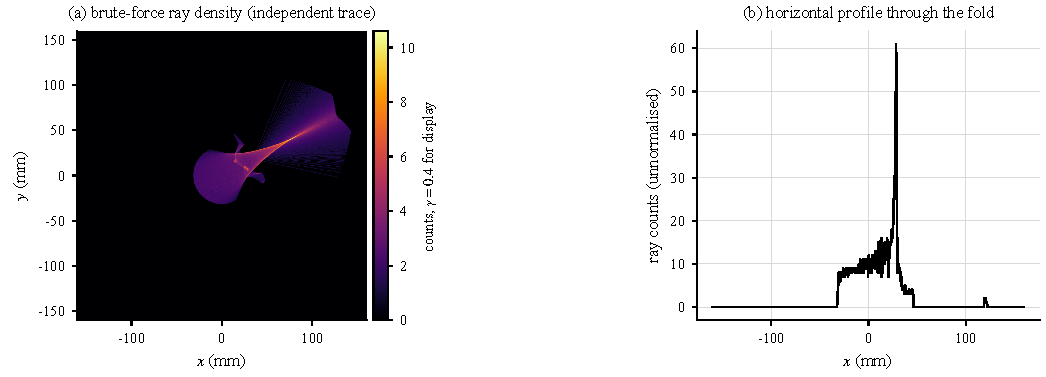
\includegraphics[width=\textwidth]{figures/fig2_fold.pdf}
\caption{The ray map of \eqref{eq:raymap}, computed by the independent
brute-force trace of Section~\ref{sec:results-quality} rather than by the
solver. The density in (a) is the caustic; the bright ridge is where
$|\detJ| \to 0$. Panel (b) cuts through it in raw ray counts. The sharpness of
that peak is what Lemma~\ref{lem:diverge} says no quadrature can bound.}
\label{fig:fold}
\end{figure*}

\subsection{The normal form of the fold, and the Airy profile}
\label{sec:foldnormal}

Lemma~\ref{lem:diverge} says the geometric answer is infinite at the fold but
says nothing about what replaces it. The replacement comes from dropping the
ray approximation and summing phases over the wavefront \cite{airy1838,berry1980}. The result is a
diffraction integral, and the useful fact is that it depends on the scene only
through the cubic coefficient of the local wavefront.

\begin{proposition}[Fold diffraction reduces to the Airy integral]
\label{prop:foldnormal}
Consider a wavefront whose phase over a one-dimensional pupil $\rho \in [-1,1]$
is
\begin{equation}
\Phi(\rho) \;=\; \frac{c\,\rho^3}{6} + x\,\rho ,
\label{eq:phase}
\end{equation}
where $c$ carries the strength of the fold and $x$ is the transverse receiver
coordinate measured from the fold. Then the field amplitude
$U(x) = \int_{-1}^{1} \exp\!\big(i\,\tfrac{2\pi}{\lambda}\Phi(\rho)\big)\dd\rho$
reduces, for $|X| \lesssim (2\pi/\lambda)^{1/3}$, to an Airy function in the
canonical coordinate
\begin{equation}
X \;=\; x\;k^{2/3}\,2^{1/3}\,c^{-1/3},
\qquad k = \frac{2\pi}{\lambda},
\label{eq:canonical}
\end{equation}
with intensity $I(x) \propto |\Ai(-X)|^2$.
\end{proposition}

\begin{proof}
Substitute $\rho = \alpha r$ with $\alpha > 0$. The phase becomes
\begin{equation}
\frac{2\pi}{\lambda}\Big( \frac{c\,\alpha^3 r^3}{6} + x\,\alpha r \Big).
\end{equation}
Choose $\alpha$ so that the cubic coefficient is $1/3$, which is the coefficient
in the Airy integral $\Ai(-X) = \frac{1}{\pi}\int_0^\infty \cos\!\big(\tfrac{t^3}{3}
- Xt\big)\dd t$:
\begin{equation}
\frac{2\pi}{\lambda}\cdot\frac{c\,\alpha^3}{6} = \frac13
\;\Longrightarrow\;
\alpha = \Big(\frac{\lambda}{\pi c}\Big)^{1/3}.
\end{equation}
The linear coefficient is then fixed, and matching it to $-X r$ gives
\begin{equation}
X \;=\; -\frac{2\pi}{\lambda}\,x\,\alpha
\;=\; -x\,2\pi^{2/3}\lambda^{-2/3}c^{-1/3}
\;=\; -x\,k^{2/3}2^{1/3}c^{-1/3},
\end{equation}
using $k^{2/3}2^{1/3} = 2\pi^{2/3}\lambda^{-2/3}$. The integral is now the Airy
integral over the scaled pupil; for $|X|$ not large the finite pupil is
immaterial because the integrand is stationary at $t = \sqrt{X}$ inside the
range, and its modulus squared is $|\Ai(-X)|^2$.
\end{proof}

\begin{remark}[Why this is the object to substitute]
\label{rem:whyairy}
Equation~\eqref{eq:canonical} is finite for every $X$, is maximal at
$X = -1.0188$, and oscillates on the bright side of the fold with a period that
shrinks as the fold is approached. Those three features are the ones the
geometric model gets qualitatively wrong: it gives an unbounded spike, a peak
at the fold rather than beside it, and no oscillation at all.
\end{remark}

\subsection{The ${\lambda^{2/3}}$ fringe scale, derived}
\label{sec:scaling}

The normal form carries exactly one length scale. Reading it off
\eqref{eq:canonical}, the transverse distance at which $|X|$ reaches order unity
is
\begin{equation}
d(\lambda,c) \;=\; k^{-2/3}\,2^{-1/3}\,c^{1/3}
\;=\; \frac{\lambda^{2/3}c^{1/3}}{2\,\pi^{2/3}} .
\label{eq:scalelaw}
\end{equation}

\begin{corollary}[Wavelength scaling]
\label{cor:scaling}
For fixed fold strength $c$, $d \propto \lambda^{2/3}$.
\end{corollary}

\begin{proof}
Immediate from \eqref{eq:scalelaw}, which contains $\lambda$ only through
$\lambda^{2/3}$.
\end{proof}

Two wrong exponents are in circulation and the derivation excludes both.
The fringe scale is not proportional to $\lambda$, which is what a naive
reading of the phase would suggest, and it is not the Fresnel
$\sqrt{\lambda}$ either; the $2/3$ comes from balancing a cubic phase against a
linear one, and either of the other exponents would come from balancing the
wrong pair of terms. The implementation uses this directly, setting the
per-channel width
\begin{equation}
w_c \;=\; w_{\text{ref}}\Big(\frac{\lambda_c}{550\,\si{\nano\meter}}\Big)^{2/3},
\qquad c \in \{R,G,B\},
\label{eq:perchannel}
\end{equation}
so chromatic separation in the fold is carried by the measured index
(Section~\ref{sec:dispersion}) together with \eqref{eq:perchannel}, and by
nothing else. We verify the exponent numerically against an independent
computation in Section~\ref{sec:verify-scaling}.

\subsection{The Airy intensity cannot be normalised by a constant}
\label{sec:notintegrable}

The correction replaces a divergent density with a profile, and the obvious way
to make that substitution conservative is to multiply by the ratio of the
integrals. That is impossible here, and the reason is a property of
$|\Ai|^2$ itself.

\begin{lemma}[The Airy intensity is not integrable on $\mathbb{R}$]
\label{lem:notl1}
$\int_{\mathbb{R}} |\Ai(-u)|^2 \dd u$ diverges. Over a truncated band
$[-L,L]$ the integral grows as $\frac{1}{\pi}\sqrt{L}$.
\end{lemma}

\begin{proof}
For $u \to +\infty$ the Airy function on the negative argument has the
oscillatory asymptotic
\begin{equation}
\Ai(-u) \;\sim\; \frac{1}{\sqrt{\pi}\,u^{1/4}}
\sin\!\Big(\frac{2}{3}u^{3/2} + \frac{\pi}{4}\Big) ,
\end{equation}
so that
\begin{equation}
|\Ai(-u)|^2 \;\sim\; \frac{1}{\pi\sqrt{u}}\,
\sin^2\!\Big(\frac{2}{3}u^{3/2} + \frac{\pi}{4}\Big) .
\end{equation}
The phase advances rapidly relative to the envelope, so the mean of the
oscillating factor is $1/2$, giving a mean intensity
$\sim (2\pi\sqrt{u})^{-1}$. Hence
\begin{equation}
\int_{1}^{L} \frac{\dd u}{2\pi\sqrt{u}} \;=\; \frac{\sqrt{L}-1}{\pi}
\;=\; \frac{1}{\pi}\sqrt{L} + \order{1} ,
\end{equation}
which is unbounded as $L \to \infty$.
\end{proof}

\begin{remark}[This is the normalisation that does not exist]
\label{rem:normdoesnotexist}
Lemma~\ref{lem:notl1} rules out the natural construction. There is no constant
$Z$ with $\frac{1}{Z}|\Ai(-u)|^2$ a probability density on $\mathbb{R}$, so a
band correction cannot be written as a profile times a global constant. What
\emph{can} be done is to conserve the band's own flux discretely, because
Corollary~\ref{cor:integrable} guarantees the band holds finite power. That is
the construction we use
(Section~\ref{sec:ours-normalisation}) and it is why the correction carries a
measured ratio rather than a closed-form constant.
\end{remark}

Table~\ref{tab:airyfacts} collects the constants used later, each evaluated
numerically rather than quoted from a table.
\begin{table}[t]
\centering
\caption{Airy quantities used in the implementation, all evaluated numerically
in this work (\texttt{scipy.special.airy}) rather than taken from a printed
table. The peak height is the normaliser in \eqref{eq:profile}; the divergence
row is Lemma~\ref{lem:notl1} at $L = 5000$.}
\label{tab:airyfacts}
\small
\begin{tabular}{@{}lll@{}}
\toprule
Quantity & Value & Note \\
\midrule
$\arg\max_u\,|\Ai(-u)|^2$            & \num{1.01879297}  & peak position \\
$\max_u |\Ai(-u)|^2$                 & \num{0.286928}    & normaliser \\
$\int_0^{\infty}\Ai(u)^2\,\dd u$     & \num{0.0669875}   & convergent half-line \\
$\int_{-L}^{80}\Ai(u)^2\,\dd u$, $L{=}5000$ & \num{22.7437} & vs.\ $\pi^{-1}\sqrt{L} = \num{22.51}$ \\
mean tail intensity                 & $(2\pi\sqrt{u})^{-1}$ & Lemma~\ref{lem:notl1} \\
\bottomrule
\end{tabular}
\end{table}

\begin{figure*}[t]
\centering
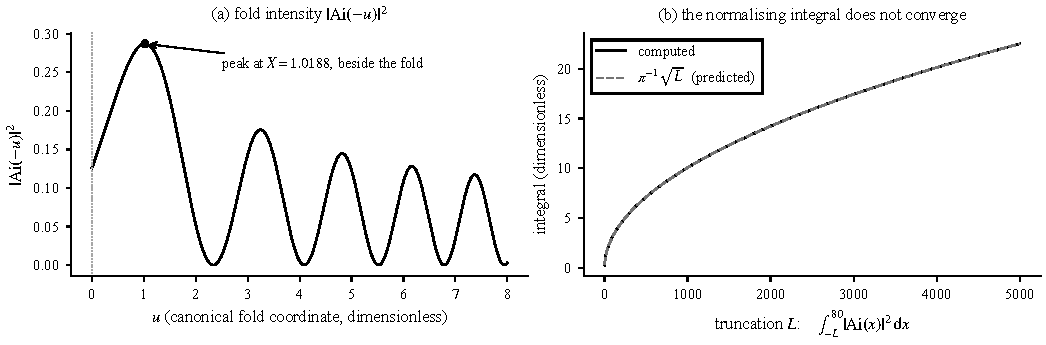
\includegraphics[width=\textwidth]{figures/fig3_airy.pdf}
\caption{Panel (a): the fold intensity $|\Ai(-u)|^2$ used by the correction
\eqref{eq:profile}, computed with \texttt{scipy.special.airy}. It is bounded,
peaks at $X = 1.0188$ \emph{beside} the fold rather than on it, and its
oscillations tighten toward the fold. Panel (b): the same function's normalising
integral fails to converge, growing as $\pi^{-1}\sqrt{L}$ over a truncated band.
That is Lemma~\ref{lem:notl1}, and it is why the correction is a discrete band
ratio \eqref{eq:kstar} rather than a constant.}
\label{fig:airy}
\end{figure*}

\subsection{The profile as implemented}
\label{sec:profile}

The implementation works in the signed distance $s$ to the detected fold and
uses a peak-normalised profile,
\begin{equation}
P(s;w) \;=\; \big|\Ai(-s/w)\big|^2 \Big/ \max_u |\Ai(-u)|^2 ,
\qquad
b(s) \;=\; 0.15 + 0.85\,P(s;w) .
\label{eq:profile}
\end{equation}
The normaliser is the $0.286928$ of Table~\ref{tab:airyfacts}, and it is a
\emph{peak} normalisation rather than an integral one because
Lemma~\ref{lem:notl1} forbids the latter. The additive floor $0.15$ keeps the
band's skirt continuous with the geometric field outside it; without it the
profile would fall to zero at the band edge and print a visible seam. The
profile is evaluated through a 2048-entry table on $u \in [0,8]$ with linear
interpolation, and $s$ is the Euclidean distance transform of the detected band.

\subsection{Dispersion, from measured data}
\label{sec:dispersion}

Both media are evaluated from measured refractive-index data rather than from
fitted dispersion formulas, for a reason that Section~\ref{sec:verify-index}
documents: a fitted curve is where this project's one physical error hid.
Water uses the four-term Sellmeier form of Daimon and Masumura
\cite{daimon2007} for HPLC-distilled water at \SI{20.0}{\celsius},
\begin{equation}
n^2(\lambda) \;=\; 1 + \sum_{j=1}^{4} \frac{B_j\,\lambda^2}{\lambda^2 - C_j},
\label{eq:sellmeier}
\end{equation}
with $\lambda$ in micrometres and the tabulated coefficients. Glass uses the
soda-lime silica form of Rubin \cite{rubin1985},
\begin{equation}
n(\lambda) \;=\; 1.5130 - 0.003169\,\lambda^2 + \frac{0.003962}{\lambda^2}.
\label{eq:rubin}
\end{equation}
At the three render channels, \eqref{eq:sellmeier} gives
$n = 1.33167 / 1.33468 / 1.33961$ and \eqref{eq:rubin} gives
$1.52104 / 1.52514 / 1.53192$. Red has the lowest index and therefore refracts
least, so red must land farthest from the axis. The chromatic ordering in every
figure of this paper is a consequence of \eqref{eq:sellmeier}, \eqref{eq:rubin}
and \eqref{eq:perchannel}, not an effect we added.

\begin{remark}[The coherence scale]
\label{rem:coherence}
The source subtends \SI{0.53}{\degree}, which at the receiver distance of this
scene corresponds to a geometric blur of roughly \SI{925}{\micro\meter}. The
physical fringe spacing implied by \eqref{eq:scalelaw} for this geometry is
\SI{123}{\micro\meter}, about \num{7.5} times smaller. A fully incoherent
treatment would therefore wash the fringes out, and the honest statement about
the fringes in this paper is that they are a \emph{resolvable wave feature of
the coherent-limit model}, not a prediction of what a photograph under the sun
would show. Section~\ref{sec:limits-coherence} treats this as the method's principal
limitation.
\end{remark}

\subsection{Fresnel transport}
\label{sec:fresnel}

Where the full scene is rendered the light path is walked through every
interface --- air, glass, water, glass, air, receiver --- with \eqref{eq:snell}
at each, and each ray carries its unpolarised Fresnel power transmission
\begin{equation}
T(c_i,\eta) \;=\; 1 - \frac12\Bigg[
\Big(\frac{\eta c_i - c_t}{\eta c_i + c_t}\Big)^{2}
+ \Big(\frac{c_i - \eta c_t}{c_i + \eta c_t}\Big)^{2} \Bigg],
\qquad c_t = \sqrt{1 - \eta^2(1-c_i^2)} .
\label{eq:fresnel}
\end{equation}
Multiplying \eqref{eq:fresnel} along each path gives the weight used by the
energy audit of Section~\ref{sec:verify-energy}, which is the non-circular
measurement that the flux ratio of Section~\ref{sec:ours-normalisation} cannot
supply on its own.

\subsection{Estimators}
\label{sec:estimators}

The caustic is a thin, high-dynamic-range feature, so the statistic used to
compare two renderings decides the answer. Two of our own earlier claims died
here rather than in the physics, and both are reported in
Section~\ref{sec:verify}. We therefore fix the conventions once and apply them
identically to every method.

\begin{itemize}
\item \textbf{Tiled correlation.} Pearson correlation against an external
reference, computed on $k \times k$ pixel tiles and reported by tile
\emph{size}. The opposite convention, indexing by tile count, silently inverted
a trend in an earlier draft
(Section~\ref{sec:verify-metric}).
\item \textbf{Edge radius.} The outermost \SI{1}{\milli\meter} annulus whose
mean channel intensity exceeds $\SI{2}{\percent}$ of that channel's own maximum.
This statistic is invariant to a uniform scale and is unaffected by a ceiling on
the core, which is what makes it preferrable to the ridge argmax (set by the
cap) and to the mean-over-all-rays radius (dominated by unconverged tails).
\item \textbf{Positive-part differential.} An isolate formed as
$\text{optics} - \text{no-optics}$ is not non-negative, because removing the
glass also removes its shadow. It is scored on its positive part, which is the
caustic. Section~\ref{sec:verify-metric} documents the factor-of-two error this
convention prevents.
\item \textbf{Temporal flicker.} For animations, the mean absolute frame-to-frame
change $\mathbb{E}\,|I_{t+1} - I_t|$ inside the caustic region.
\end{itemize}

\begin{remark}[On the word ``converged'']
\label{rem:converged}
Used in this paper it means the resource budget was exhausted and the statistic
had stopped moving at the reported precision. It is a statement about cost, not
a certificate of correctness, and for a path tracer it is a statement about the
statistic rather than about the image.
\end{remark}
